\documentclass[a4paper,12pt]{article} 
% 使用ctex包支持中文
\usepackage{ctex}
% 开始文档
\usepackage{color}
\usepackage{graphicx}
\begin{document}

% 创建标题页的内容
\title {八省联考导数压轴}
\author{潘世维}
\date{Friday, 20 October 2021}
\maketitle

已知函数 $ f(x)=e^{x}-\sin x-\cos x, g(x)=e^{x}+\sin x+\cos x$


(1) 证明: 当 $ x>-\frac{5 \pi}{4}  时,  f(x) \geq 0 $



(2) 若 $ g(x) \geq 2+a x $, 求  a 
\begin{flushleft}
~\\
\textcolor{red}{证法1:}\\
证明$e^x \ge \sin x + \cos x = \sqrt 2 \sin \left( x + \frac{\pi }{4} \right) $
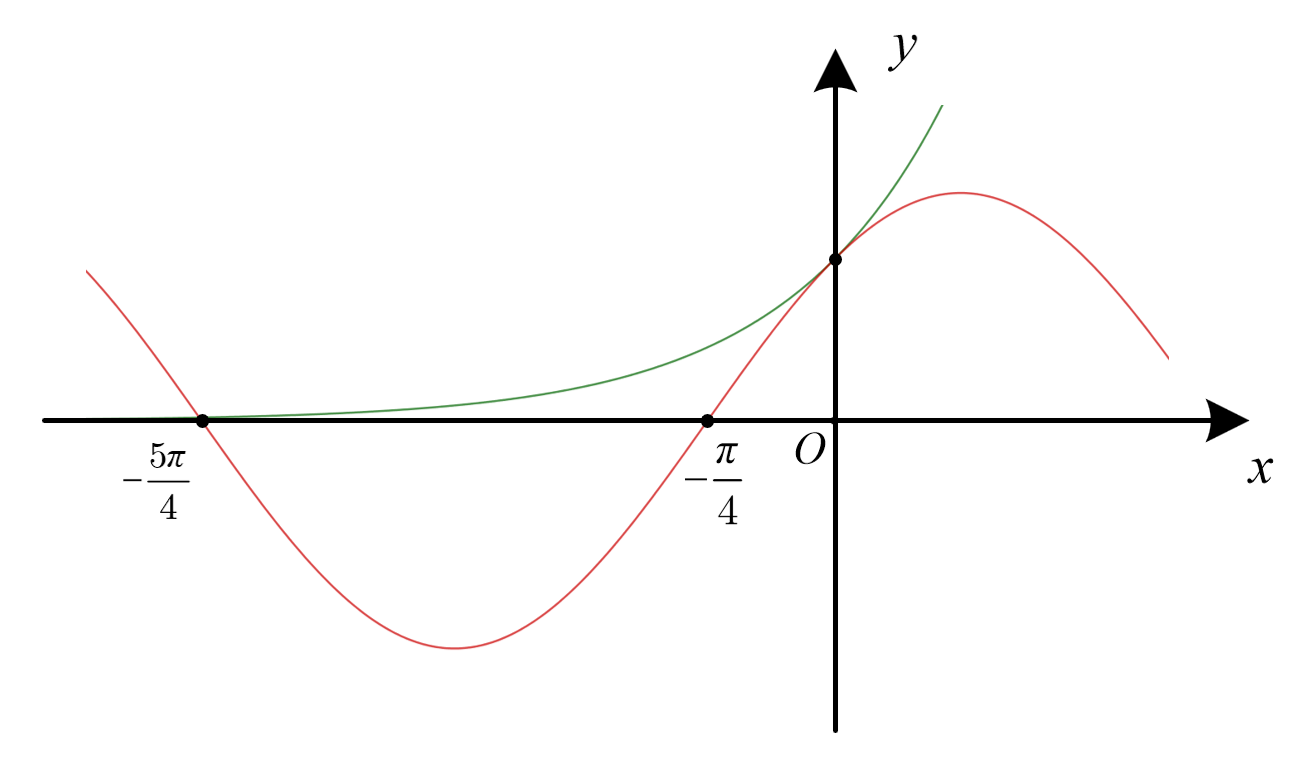
\includegraphics[scale=0.2]{D:/OneDrive/document/8 provinces/pic/pic1.png}\\
①

\end{flushleft}
\end{document}  